% \documentclass[ba,preprint]{imsart}% use this for supplement article
\documentclass[ba]{imsart}
%
\pubyear{2022}
\volume{TBA}
\issue{TBA}
\doi{0000}
\arxiv{2010.00000}
\firstpage{1}
\lastpage{1}

%
\usepackage{amsthm}
\usepackage{amsmath}
\usepackage{amssymb}
\usepackage{xcolor}
\usepackage{bm}
\usepackage{natbib}
\usepackage[
  colorlinks,
  citecolor=blue,
  urlcolor=blue,
  filecolor=blue,
  backref=page
]{hyperref}
\usepackage{graphicx}

%% Comentarios
\usepackage{todonotes}
\usepackage{ulem}

\startlocaldefs
\numberwithin{equation}{section}
\theoremstyle{plain}
\newtheorem{theorem}{Theorem}[section]
\newtheorem{proposition}{Proposition}[section]

\renewcommand{\epsilon}{\varepsilon}

\newcommand{\N}{\mathbb{N}}
\newcommand{\R}{\mathbb{R}}
\newcommand{\E}{\mathbb{E}}
\newcommand{\Hcal}{\ensuremath\mathcal{H}}
\newcommand{\Var}{\ensuremath\operatorname{Var}}
\definecolor{violet}{rgb}{0.7,0,0.6}

%% Scalar product
\newcommand\dotprod[2]{\left\langle #1, #2 \right\rangle}

%% Colors
\definecolor{comment-red}{RGB}{240,30,70}

%% Environment for colored comments
\newenvironment{comment}[1][comment-red]
{
\noindent \color{#1}
}
{
\color{black}
}

%% Inline comments
\newcommand\incomment[2][comment-red]{\color{#1}[\textit{#2}]\color{black}}
\endlocaldefs

\begin{document}

\begin{frontmatter}
\title{Bayesian RKHS-based methods in functional regression\support{Support information of the article.}}
\runtitle{Bayesian RKHS-based methods in functional regression}

\begin{aug}
\author{\fnms{First} \snm{Author}\thanksref{addr1,t1,t2,m1}\ead[label=e1]{first@somewhere.com}},
\author{\fnms{Second} \snm{Author}\thanksref{addr1,t3,m1,m2}\ead[label=e2]{second@somewhere.com}}
\and
\author{\fnms{Third} \snm{Author}\thanksref{addr2,t1,m2}%
\ead[label=e3]{third@somewhere.com}%
\ead[label=u1,url]{http://www.foo.com}}

\runauthor{F. Author et al.}

\address[addr1]{Address of the First and Second authors
     Usually a few lines long
    \printead{e1} % print email address of "e1"
    \printead*{e2}
}

\address[addr2]{Address of the Third author
    Usually a few lines long
    Usually a few lines long
    \printead{e3}
    \printead{u1}
}

\thankstext{t1}{Some comment}
\thankstext{t2}{First supporter of the project}
\thankstext{t3}{Second supporter of the project}

\end{aug}

\begin{abstract}
We propose a novel Bayesian approach for functional linear and logistic regression models based on the theory of Reproducing Kernel Hilbert Spaces (RKHS's). These new models build upon the RKHS associated with the covariance function of the underlying stochastic process, and can be viewed as a finite-dimensional approximation to the classical functional regression paradigm. The corresponding functional model (or the functional logistic equation in the case of binary response) is determined by a function living on a dense subspace of the RKHS of interest. By imposing a suitable prior distribution on this space, we can perform data-driven inference via standard Bayes methodology, and the posterior distribution can be estimated through Markov chain Monte Carlo methods. Several prediction strategies derived from this posterior distribution turn out to be competitive against other usual alternatives in both simulated examples and real data sets, including a Bayesian-motivated variable selection procedure.
\end{abstract}

\begin{keyword}[class=MSC]
\kwd[primary ]{62M20}
\kwd[; secondary ]{62F15}
\end{keyword}

\begin{keyword}
\kwd{functional data}
\kwd{linear regression}
\kwd{logistic regression}
\kwd{reproducing kernel Hilbert space}
\kwd{Bayesian inference}
\end{keyword}

\end{frontmatter}

\section{Introduction}\label{sec:intro}

The problem of predicting a scalar response from a functional covariate is one that has gained traction over the last few decades, as more and more data is being generated with an ever-increasing level of granularity in the measurements. While in principle the functional data could be simply regarded as a discretized vector in a very high dimension, there are often many advantages in taking into account the functional nature of the data, ranging from modeling the possibly high correlation among points that are close in the domain, to extracting information that may be hidden in the derivatives of the function in question. As a consequence, numerous proposals have arisen on how to suitably deal with functional data, all of them encompassed under the term Functional Data Analysis (FDA), which essentially explores statistical techniques to process, model and make inference on data varying over a continuum. A partial survey on such techniques and methods is \citet{cuevas2014partial}, while a more detailed exposition of the theory and applications can be found for example in \citet{hsing2015theoretical} or the book by \citet{horvath2012inference}.

FDA is undoubtedly an active area of research, which finds applications in a wide variety of fields, such as biomedicine, finance, meteorology or chemistry \citep[see for example][]{ullah2013applications}. Accordingly, there are many recent contributions on how to tackle functional data problems, both from a theoretical and practical standpoint. Chief among them is the approach of reducing the problem to a finite-dimensional one, for example using a truncated basis expansion or spline interpolation methods \citep[e.g.][]{muller2005generalized, aguilera2013comparative}. At the same time, much effort has also been put into the opposite task: generalizing different concepts to the infinite-dimensional framework. Examples of this endeavor include a functional Mahalanobis distance \citep{berrendero2020mahalanobis} or a functional partial least squares algorithm \citep{delaigle2012methodology}. Another technique found in the related literature is the use of Gaussian processes to model the functional behavior of the data \citep[see for instance][]{shi2011gaussian}. These ideas extend the theory of Gaussian process regression in classical finite-dimensional settings \citep{rasmussen2004gaussian}, providing an alternative Bayesian approach to functional inference and prediction problems. Additional non-parametric methods for functional prediction and classification were notably explored in \citet{ferraty2006nonparametric}.

In this work we are concerned with functional linear and logistic regression models, that is, situations where the goal is to predict a continuous or dichotomous variable from functional observations. Even though these problems can be formally stated with almost no differences from their finite-dimensional counterparts, there are some fundamental challenges as well as some subtle drawbacks that emerge as a result of working in infinite dimensions. To set a common framework, throughout this work we will consider a scalar response variable \(Y\) (either continuous or binary) which has some dependence on a stochastic \(L^2\)-process \(X=X(t)=X(t, \omega)\) with trajectories in \(L^2[0, 1]\). We will further suppose without loss of generality that \(X\) is centered, that is to say, its mean function \(m(t)=\E[X(t)]\) vanishes for all \(t\in[0,1]\). In addition, we will tacitly assume the existence of a \textit{labeled} data set \(\mathcal D_n =\{(X_i, Y_i): i=1,\dots, n\}\) of independent observations from \((X, Y)\), and our aim will be to accurately predict the response corresponding to unlabeled samples from \(X\).

\subsubsection{\(L^2\)-models, shortcomings and alternatives}

 The most common functional linear regression model is the classical \(L^2\)-model, widely popularized since the first edition (1997) of the monograph by~\citet{ramsay2005functional}. It can be seen as a generalization of the usual finite-dimensional model, replacing the scalar product in \(\R^d\) for that of the functional space \(L^2[0,1]\):
\begin{equation}\label{eq:l2-linear-model}
Y = \alpha_0 + \dotprod{X}{\beta} + \epsilon = \alpha_0 + \int_0^1 X(t)\beta(t)\, dt + \epsilon,
\end{equation}
where \(\alpha_0\in \R\), \(\epsilon\) is a random error term independent from \(X\) with \(\E [\epsilon]=0\), and the functional slope parameter \(\beta=\beta(\cdot)\) is assumed to be a member of the infinite-dimensional space \(L^2[0, 1]\). In this case, the inference on \(\beta\) is hampered by the fact that \(L^2[0,1]\) is an extremely wide space that also contains many non-smooth or ill-behaved functions, so that any estimation procedure involving optimization on it would typically be hard. In spite of this, model~\eqref{eq:l2-linear-model} is not flexible enough to include ``simple'' finite-dimensional models based on linear combinations of the marginals, such as \(Y=\alpha_0 + \beta_1 X(t_1)+ \cdots + \beta_p X(t_p) + \epsilon\) for some constants \(\beta_j\in\R\) and instants \(t_j\in[0,1]\); see \citet{berrendero2020general} for additional details on this. Moreover, the non-invertibility of the covariance operator associated with \(X\) (defined in Section~\ref{sec:rkhs}), which plays the role of the covariance matrix in the infinite case, invalidates the usual least squares theory. Thus, some regularization or dimensionality reduction technique is needed for parameter estimation.

A similar \(L^2\)-based functional logistic equation can be derived for the binary classification problem via the logistic function:
\begin{equation}\label{eq:l2-logistic-model}
  \mathbb P(Y=1 \mid X) = \frac{1}{1 + \exp\{-\alpha_0 - \dotprod{X}{\beta}\}},
\end{equation}
where \(\alpha_0 \in \R\) and \(\beta \in L^2[0, 1]\). In this situation, the most common way of estimating the slope function \(\beta\) is via its Maximum Likelihood Estimator (MLE). However, not only do the same complications as in the linear regression model apply in this situation, but there is also the additional problem that in functional settings the MLE does not exist with probability one under fairly general conditions \citep[see][Sec.~3.2]{berrendero2018functional}.

It turns out that in both scenarios a natural alternative to the \(L^2\)-model is the so-called Reproducing Kernel Hilbert Space (RKHS) model, which instead assumes the unknown functional parameter to be a member of the RKHS associated with the covariance function of the process \(X\), making use of the scalar product of that functional space. As we will show later on, not only is this model simpler and arguably easier to interpret, but it also constrains the parameter space to smoother and more manageable functions. In fact, it includes a model based on finite linear combinations of the marginals of \(X\) as a particular case, which is especially appealing to practitioners confronted with functional data problems due to its simplicity. These RKHS-based models and their idiosyncrasies have been explored in \citet{berrendero2019rkhs, berrendero2020general} in the functional linear regression setting, and in \citet{berrendero2018functional, berrendero2018use} for the case of functional logistic regression. Incidentally, these models also shed light on the near-perfect classification phenomenon for functional data, described by \citet{delaigle2012achieving} and further examined for example in the works of \citet{berrendero2018use} or \citet{torrecilla2020optimal}.

A major aim of this work is to motivate these recently-proposed models inside the functional framework, while also providing efficient techniques to apply them in practice. Our main contribution is the proposal of a Bayesian approach to parameter estimation within the aforementioned RKHS models, in which a prior distribution is imposed on the unknown functional parameter to obtain a posterior distribution after seeing the data. Although setting a prior distribution on a function space is generally a hard task, the specific parametric formulation of the RKHS models we propose greatly facilitates this (see Section~\ref{sec:methodology} for details). A similar Bayesian scheme has recently been explored in \citet{grollemund2019bayesian}, albeit not within a RKHS framework.

Another set of techniques extensively studied in this context are variable selection methods, which aim to select the marginals \(\{X(t_j)\}\) of the process that better summarize it according to some optimality criterion. As it happens, some variable selection methods have already been proposed in the RKHS framework \citep[see for example][]{berrendero2019rkhs}, but in general they have their own dedicated algorithms and procedures. As will become apparent in the forthcoming sections, given the nature of our suggested Bayesian model we can easily isolate the marginal posterior distribution corresponding to a finite set of points \(\{t_j\}\), and thus provide a Bayesian-motivated variable selection process along with the other prediction methods that naturally arise within our model. In this way, in addition to making predictions about the input data, we can evaluate exactly which marginals of the functional explanatory variable contain the most relevant information. These points-of-impact selection models for functional predictors have also been considered in the  literature; see \citet{poss2020superconsistent}, \citet{berrendero2016variable} or \citet{ferraty2010most} by way of illustration. Another example of a related strategy is the work of \citet{james2009functional}, in which the authors propose a method to estimate \(\beta(t)\) in such a way that it is exactly zero over some regions in the domain.

\subsubsection{Organization of the paper}

In Section~\ref{sec:rkhs} we review the basics of the theory of RKHS's from a probabilistic point of view. Section~\ref{sec:methodology} is devoted to explaining the Bayesian methodology and the functional regression models we propose. The empirical results of the experimentation are contained in Section~\ref{sec:results}, which also includes a short discussion of computational details. Lastly, the conclusions drawn from this work are presented in Section~\ref{sec:conclusion}.

\subsection{Some essentials on RKHS's and notation}\label{sec:rkhs}

The methodology proposed in this work relies heavily on the use of RKHS's, so before diving into it we will briefly describe the main characteristics of these spaces (for a more detailed account, see for example~\citet{berlinet2004reproducing}). Let us denote by \(K(t, s)= \mathbb E[X(t)X(s)]\) the covariance function of the centered process \(X\), and in what follows suppose that it is continuous. To construct the RKHS \(\Hcal(K)\) associated with the covariance function, we start by defining the functional space \(\Hcal_0(K)\) of all finite linear combinations of evaluations of \(K\), that is,
\begin{equation}\label{eq:h0}
\Hcal_0(K) = \left\{ f \in L^2[0,1]: \ f(\cdot) = \sum_{i=1}^p a_i K(t_i, \cdot), \ p \in \N, \ a_i \in \R, \ t_i \in [0, 1] \right\}.
\end{equation}
This space is endowed with the inner product \(\dotprod{f}{g}_K = \sum_{i, j} a_i b_j K(t_i, s_j)\), given that \(f(\cdot)=\sum_i a_i K(t_i, \cdot) \) and \(g(\cdot)=\sum_j b_j K(s_j, \cdot)\). Then, \(\Hcal(K)\) is defined to be the completion of \(\Hcal_0(K)\) under the norm induced by the scalar product \(\dotprod{\cdot}{\cdot}_K\). As it turns out, functions in this space satisfy the \textit{reproducing property} \(\dotprod{K(t, \cdot)}{f}_K = f(t)\) for all \(f \in \Hcal(K)\) and \(t \in [0, 1]\). An important consequence is that \(\Hcal(K)\) is a space of genuine functions and not of equivalence classes, since the values of the functions at particular points are in fact relevant, unlike in \(L^2\)-spaces.

Note that he covariance function of \(X\) (sometimes referred to as the \textit{kernel}) plays a crucial role in characterizing the RKHS. An integral operator closely related to this kernel is the so-called covariance operator, namely \(\mathcal Kf(\cdot) = \int_0^1 K(s, \cdot)f(s)\, ds\) for \(f \in L^2[0, 1]\), which is self-adjoint and compact when \(K\) is continuous \citep[e.g.][Th.~4.6.2]{hsing2015theoretical}. It is worth mentioning that this operator provides several alternative definitions of \(\Hcal(K)\); for example, the RKHS can be identified with the image of the square root of the covariance operator, i.e., \(\Hcal(K) = \mathcal K^{1/2}(L^2[0, 1])\), with inner product \(\dotprod{f}{g}_K = \dotprod{\mathcal K^{-1/2}(f)}{\mathcal K^{-1/2}(g)}\). Furthermore, we can think of the norm in \(\Hcal(K)\) as an \(L^2\)-like regularized norm, since this space can be seen as \(\Hcal(K) = \{f \in L^2[0, 1]: \ \sum_j \lambda_j^{-1}\dotprod{f}{\phi_j}^2 < \infty \}\), where \(\lambda_j\) and \(\phi_j\) are the eigenvalues and (orthonormal) eigenfunctions of \(\mathcal K\), respectively. In this case, the corresponding inner product is \(\dotprod{f}{g}_K = \sum_j \lambda_j^{-1}\dotprod{f}{\phi_j}\dotprod{g}{\phi_j}\). Note that, since the spectral theorem for compact operators tells us that the sequence of eigenvalues \(\{\lambda_j\}\) tends to zero \citep[e.g.][Th.~4.2.4]{hsing2015theoretical}, this definition highlights the fact that functions in \(\Hcal(K)\) are smooth, in the sense that their components in an orthonormal basis need to vanish quickly.

Lastly, a particularly useful approach in statistics is to regard \(\Hcal(K)\) as an isometric copy of a well-known space. Specifically, via \textit{Loève's isometry} \citep{loeve1948fonctions} one can establish a congruence \(\Psi_X\) between \(\Hcal(K)\) and the linear span of the process, \(\mathcal L(X)\), in the space of all random variables with finite second moment, \(L^2(\Omega)\) \citep[see Lemma 1.1 in][]{lukic2001stochastic}. This isometry is essentially the completion of the correspondence
  \begin{equation}\label{eq:loeves-isometry}
  \sum_{i=1}^p a_i X(t_i) \longleftrightarrow \sum_{i=1}^p a_i K(t_i, \cdot),
  \end{equation}
and can be formally defined, in terms of its inverse, as \(\Psi^{-1}_X(U)(t) = \E[U X(t)]\) for \(U \in \mathcal L(X)\).
Despite the close connection between the process \(X\) and the space \(\Hcal(K)\), special care must be taken when dealing with concrete realizations of the process, since under rather general conditions the trajectories of \(X\) do not belong to the corresponding RKHS with probability one \citep[see for example][Cor.~7.1]{lukic2001stochastic}. As a consequence, the expression \(\dotprod{x}{f}_K\) is ill-defined and lacks meaning when \(x\) is a realization of \(X\). However, following Parzen's approach in his seminal work \citep[e.g.][Th.~4E]{parzen1961approach}, we can leverage Loève's isometry and identify \(\dotprod{x}{f}_K \) with the image \( \Psi_x(f) := \Psi_X(f)(\omega)\), for \(x=X(\omega)\) and \(f\in \Hcal(K)\). This notation, viewed as a formal extension of the inner product, often proves to be useful and convenient.

\section{Bayesian methodology for RKHS-based functional regression models}\label{sec:methodology}

In this section we present the precise models and Bayesian methodologies explored in this work. The RKHS-based functional models under consideration \citep[see][]{berrendero2018functional, berrendero2019rkhs} are those obtained by taking a functional parameter \(\alpha \in \Hcal(K)\) and replacing the scalar product for \(\dotprod{X}{\alpha}_K\) in the \(L^2\)-models~\eqref{eq:l2-linear-model} and~\eqref{eq:l2-logistic-model}. However, to further simplify things we will follow a parametric approach and suppose that \(\alpha\) is in fact a member of the dense subspace \(\Hcal_0(K)\) defined in~\eqref{eq:h0}. For practical and computational reasons, the value of \(p\), the dimensionality of the model, will be fixed beforehand in a suitable way (see Section~\ref{sec:model-choice} for details), and we will regard \(\beta_j\) and \(t_j\) as free parameters. Thus, we will search for our functional parameter in the set
\begin{equation}\label{eq:h0p}
\Hcal_{0,p}(K)=\left\{ \sum_{j=1}^p \beta_j K(t_j, \cdot): \ \beta_j \in \R, \ t_j \in [0, 1]\right\}.
\end{equation}

The general idea will be to impose a prior distribution on these free parameters (and possibly others) to eventually derive a posterior model after incorporating the available sample information.  Moreover, as we said before, with a slight abuse of notation we will understand the expression \(\dotprod{x}{\alpha}_K\) as \(\Psi_x(\alpha)\), where \(x=X(\omega)\) and \(\Psi_x\) is Loève's isometry. Hence, taking into account that \(\alpha \in \Hcal_{0,p}(K)\) and that \(\Psi_X(K(t, \cdot)) = X(t)\) by definition (see~\eqref{eq:loeves-isometry}), we can write \(\dotprod{x}{\alpha}_K \equiv \sum_j \beta_j x(t_j)\) when \(\alpha(\cdot)=\sum_j\beta_j K(t_j, \cdot)\).

In view of~\eqref{eq:h0p}, to set a prior distribution on the unknown function \(\alpha\) (that is, a prior distribution on the functional space \(\Hcal_{0,p}(K)\)) it suffices to consider \(p\)-dimensional continuous prior distributions for the coefficients \(\beta_j\) and the times \(t_j\) separately. Thanks to this parametric approach, the challenging task of setting a prior distribution on a space of functions is considerably simplified, while simultaneously not constraining the model to any specific distribution (in contrast to, for instance, Gaussian process regression methods). Moreover, note that starting from a probability distribution \(\mathbb{P}_0\) on \(\Hcal_0(K)\) we can obtain a probability distribution \(\mathbb{P}\) on \(\Hcal(K)\) merely by defining \(\mathbb{P}(B) = \mathbb{P}_0(B\cap \Hcal_0(K))\) for all Borel sets \(B\). Consequently, our simplifying assumption on \(\alpha\) is not very restrictive, since any prior distribution on \(\Hcal_0(K)\) can be directly extended to a prior distribution on \(\Hcal(K)\). Even though we actually work on \(\Hcal_{0,p}(K)\), the discrete parameter \(p\) can still be selected in several meaningful ways that make use of the available data, and the set of feasible values is not very large in practice.

In any case, after selecting a suitable prior distribution \(\pi(\theta)\) for the finite-dimensional parameter vector \(\theta\), we can resort to Bayes' theorem to perform the inference step, which in the case of i.i.d. samples amounts to
\begin{equation}\label{eq:bayes-theorem}
  \pi(\theta \mid \mathcal D_n) \propto \left( \prod_{i=1}^n \pi(Y_i\mid X_i, \theta) \right)\pi(\theta).
\end{equation}
In Sections~\ref{sec:rkhs-linear-model} and~\ref{sec:rkhs-logistic-model} we proceed to specify the parameter spaces, prior distributions and concrete models for \(\pi(Y | X,\theta)\) considered in the case of functional linear regression and functional logistic regression, respectively. Even though in~\eqref{eq:bayes-theorem} we have omitted the possibly intractable integral related to the normalizing constant, sampling from the (approximate) posterior distribution can be accomplished via Markov Chain Monte Carlo (MCMC) methods \citep[e.g.][]{brooks2011handbook}. Note that the use of MCMC algorithms introduces a source of stochasticity in the prediction procedure.

\subsection{Functional linear regression}\label{sec:rkhs-linear-model}

In the case of functional linear regression, the simplified RKHS model considered in this work is given by
\begin{equation}\label{eq:rkhs-model-linear}
  Y = \alpha_0 + \Psi_X(\alpha) + \epsilon = \alpha_0 + \sum_{j=1}^p \beta_j X(t_j) + \epsilon,
\end{equation}
where \(\alpha(\cdot)=\sum_{j=1}^p\beta_jK(t_j, \cdot) \in \Hcal_{0,p}(K), \beta_j \in \R\), \(t_j \in [0, 1]\), \(\alpha_0\in\R\), and \(\epsilon\) is a normally-distributed error term independent from \(X\), with \(\E[\epsilon]=0\) and \(\Var(\epsilon)=\sigma^2\in \R^+\). This model is essentially a finite-dimensional approximation from a functional perspective to the more general RKHS model that assumes \(\alpha \in \Hcal(K)\), proposed in~\citet{berrendero2019rkhs}.

When \(p\) is fixed, the parameter space of dimension \(2p + 2\) becomes \(\Theta_p = \R^p \times [0, 1]^p \times \R \times \R^+\), and in the sequel a generic element of this space will be denoted by \(\theta = (\beta_1,\dots, \beta_p, t_1,\dots, t_p, \alpha_0, \sigma^2) \equiv (b, \tau, \alpha_0, \sigma^2)\). Before proceeding any further, observe that we can rewrite model~\eqref{eq:rkhs-model-linear} in a more explicit and practical fashion in terms of the available sample information in \(\mathcal D_n\). For \(\theta \in \Theta_p\), the reinterpreted model assumes the form
\begin{equation}\label{eq:rkhs-model-linear-2}
  Y_i \mid X_i, \theta \ \stackrel{\text{i.i.d.}}{\sim} \mathcal N\left(\alpha_0 + \sum_{j=1}^p \beta_j X_i(t_j), \ \sigma^2\right), \quad i =1,\dots, n.
\end{equation}

It is worth mentioning that the model remains linear in the sense that it fundamentally involves a random variable belonging to the linear span of the process \(X\) in \(L^2(\Omega)\). Also, note that given the time instants \(t_j\), the model becomes a multiple linear model with the \(X(t_j)\) as scalar covariates. As a matter of fact, this RKHS model is particularly suited as a basis for variable selection methods, and also entails the classical \(L^2\)-model~\eqref{eq:l2-linear-model} under certain conditions \citep[see][Sec.~3]{berrendero2020general}. In addition, this model could be easily extended to the case of several covariates via an expression of type \(Y=\alpha_0 + \Psi_{X^{1}}(\alpha_1) + \cdots + \Psi_{X^{q}}(\alpha_q) + \epsilon\). In that case, as argued in \citet{grollemund2019bayesian} for a similar situation, if we were to set a prior distribution on all the parameters involved, we could recover the full posterior by looking alternately at the posterior distribution of each covariate conditional on the rest of them.

\subsubsection{The bayesian approach: prior selection and posterior derivation}

The prior distribution suggested for the parameter vector \(\theta \in \Theta_p\) is given by
\begin{align}\label{eq:prior-linear}
  \begin{split}
  \pi(\alpha_0, \sigma^2)              & \propto 1/\sigma^2,                                                     \\
  \tau                     & \sim \mathcal U([0, 1]^p),                                              \\
  b\mid \tau, \sigma^2 & \sim \mathcal N_p(b_0, g\sigma^2{\underbrace{\left(\mathcal X_\tau' \mathcal X_\tau + \eta I\right)}_{G_\tau}}^{-1}),
\end{split}
\end{align}
where \(I\) is the identity matrix, \(\mathcal X_\tau\) is the data matrix \((X_i(t_j))_{i,j}\), and \(b_0\in \R^p, \ g \in \R\) and \(\eta \in \R^+\) are hyperparameters of the model. On the one hand, note the use of a joint prior distribution on \(\alpha_0\) and \(\sigma^2\), which is a widely used non-informative prior known as Jeffrey's prior \citep{jeffreys1946invariant}. In any event, the estimation of \(\alpha_0=\E[Y]\) is straightforward, so it could have been left out of the model altogether. On the other hand, the prior on \(b\) is a slight modification of the well-known Zellner's g-prior \citep{zellner1986assessing}, in which a regularizing term is added to avoid ill-conditioning problems in the Gram matrix, obtaining a ridge-like Zellner prior controlled by the tuning parameter \(\eta\) \citep{baragatti2012study}. All in all, with a slight abuse of notation the proposed prior distribution becomes \(\pi(\theta) = \pi(b| \tau, \sigma^2)\pi(\tau)\pi(\alpha_0, \sigma^2)\).

As for the posterior distribution, we only compute a function proportional to its log-density, since that is all that is needed for the MCMC algorithm to work. A standard algebraic manipulation in~\eqref{eq:bayes-theorem} yields the following result.

\begin{proposition}
Under the linear model~\eqref{eq:rkhs-model-linear-2}, the prior distribution implied in~\eqref{eq:prior-linear} produces the log-posterior distribution
\begin{align*}
\log \pi(\theta \mid \mathcal D_n) \propto {} & \frac{1}{2\sigma^2}\left(\|\bm Y- \alpha_0\bm{1} - \mathcal X_\tau b\|^2 + \frac{1}{g}(b - b_0)'G_\tau(b - b_0) \right)\\
& + (p+n+2)\log\sigma - \frac{1}{2}\log |G_\tau|,
\end{align*}
where \(\bm Y=(Y_1,\dots,Y_n)'\) and \(\bm{1}\) is an \(n\)-dimensional vector of ones.
\end{proposition}

\subsubsection{Making predictions}

In order to generate predictions, let us recall that when performing the empirical posterior approximation, on each of the \(M\) steps of the iterative MCMC algorithm we get an approximate sample \(\theta^{(m)*}=(b^{(m)*}, \tau^{(m)*}, \alpha_0^{(m)*}, (\sigma^2)^{(m)*})\) of the posterior distribution \(\pi(\theta| \mathcal D_n)\). Assuming now a previously unseen test set \(\mathcal D'_{n'}\) in the same conditions as \(\mathcal D_n\), we propose to construct three different kinds of predictors based on the MCMC samples, each of them following a different strategy.

\begin{description}
  \item[Summarize-then-predict.] If we consider a point-estimate statistic \(T\) to act as a summary of the posterior distribution, we can get the corresponding estimates \(\hat{\theta}=(\hat b, \hat \tau, \hat{\alpha}_0, \hat{\sigma}^2) = T\{\theta^{(m)*}\} \equiv (T\{b^{(m)*}\}, T\{\tau^{(m)*}\}, T\{\alpha_0^{(m)*}\}, T\{(\sigma^2)^{(m)*}\})\) and predict the responses in the usual way following model \eqref{eq:rkhs-model-linear}, i.e.:
  \[
    \hat Y_i = \hat{\alpha}_0 + \sum_{j=1}^p \hat{\beta}_j X_i(\hat{t}_j), \quad i=1,\dots, n'.
  \]
  Note that in this case the variance \(\sigma^2\) is treated as a nuisance parameter. Although it contributes to measure the uncertainty in the approximations, its estimates are discarded in the final prediction.

  \item[Predict-then-summarize.] Alternatively, we can  look at the approximate posterior distribution as a whole and compute the predictive distribution of the simulated responses at each step of the chain following model~\eqref{eq:rkhs-model-linear-2}:
  \begin{equation}\label{eq:sampled-response-vector}
  \bm Y^{(m)*} := \left\{Y_i^{(m)*} \equiv Y_i \mid X_i, \theta^{(m)*}:\ i=1,\dots,n'\right\}, \quad m=1,\dots,M.
  \end{equation}
  Then, we can take the mean of all such simulated responses as a proxy for each response variable, that is,
  \[
  \hat Y_i = \frac{1}{M}\sum_{m=1}^M Y_i^{(m)*}, \quad i=1,\dots,n'.
  \]
  This method differs from the previous one in that it takes into account the full approximate posterior distribution instead of summarizing it directly.

  \item[Variable selection.] Lastly, we can focus only on the marginal posterior distribution of \(\tau|\mathcal D_n\) and select \(p\) time instants using a point-estimate statistic \(T\) as in our first strategy, but discarding the rest of the parameters. Specifically, we can consider the times \(\hat t_j = T\{t_j^{(m)*}\}\) and reduce the original data set to just the \(n\times p\) real matrix \(\{X_i(\hat t_j): i=1, \dots,n, \ j=1,\dots,p\}\). After this variable selection has been carried out, we can tackle the problem using a finite-dimensional linear regression model and apply any of the well-known prediction algorithms suited for this situation.
\end{description}

Note that these predictors can be obtained all at once after only one round of training (that is, an individual MCMC run to approximate the posterior distribution). As a consequence, what we have in practice is a single algorithm that can produce multiple predictors at the same computational cost, so that any of them can be chosen (or even switched back and forth) depending on the particularities of the problem at hand. Moreover, one could even contemplate an \textit{ensemble model} in which some kind of aggregation of several of the available prediction methods is performed to produce a final result.

\subsection{Functional logistic regression}\label{sec:rkhs-logistic-model}

In the case of functional logistic regression, we regard the binary response variable \(Y\in\{0, 1\}\) as a Bernoulli random variable given the regressor \(X=x \in L^2[0, 1]\), and suppose that \(\log\left(p(x)/(1-p(x))\right)\) is linear in \(x\), where \(p(x)=\mathbb P(Y=1| X=x)\). Then, following the approach  suggested by \citet{berrendero2018functional}, an RKHS model might be given  by the  equation
\begin{equation}\label{eq:rkhs-model-logistic}
  \mathbb P(Y=1 \mid X) = \frac{1}{1 + \exp\{-\alpha_0 - \Psi_X(\alpha)\}}, \quad \alpha_0 \in \R, \ \alpha \in \Hcal_{0,p}(K).
\end{equation}

Indeed, note that this can be seen as a finite-dimensional approximation (but, still, with a functional interpretation) to the general RKHS functional logistic model proposed by these authors, which can be obtained by replacing \(\Hcal_{0,p}(K)\) with the whole RKHS space \(\Hcal(K)\). Now, if we aim at a classification problem, our strategy will be similar to that followed in the functional linear model: after incorporating the sample information, we can rewrite~\eqref{eq:rkhs-model-logistic} as
\begin{equation}\label{eq:rkhs-model-logistic-2}
Y_i \mid X_i,\theta \ \stackrel{\text{i.i.d.}}{\sim} \operatorname{Bernoulli}(p_i), \quad i=1,\dots, n,
\end{equation}
with
\begin{equation}\label{eq:rkhs-model-logistic-2-parameter}
  p_i = \mathbb P(Y_i=1 \mid X_i,\theta) = \frac{1}{\displaystyle 1 + \exp\left\{-\alpha_0 - \sum_{j=1}^p \beta_j X_i(t_j)\right\}}, \quad i=1,\dots, n,
\end{equation}
where in turn \(\beta_j\in\R\) and \(t_j\in[0, 1]\).

In much the same way as the linear regression model described above, this RKHS-based logistic regression model offers some advantages over the \(L^2\)-model. First and foremost, it has a more straightforward interpretation and allows for a workable Bayesian approach, as we will demonstrate below. Secondly, it can be shown that under mild conditions the general RKHS logistic functional model holds whenever the conditional distributions \(X | Y=i\) (\(i=0,1\)) are homoscedastic Gaussian processes~\citep[see Theorem 1 in][]{berrendero2018functional}; this provides a sound theoretical motivation for such model. Furthermore, a maximum likelihood approach for parameter estimation (although not considered here) is possible as well. Indeed, the use of a finite-dimensional approximation  mitigates the problem of non-existence of the MLE in the functional case. However, let us recall that even in finite-dimensional settings there are cases of quasi-complete separation in which the MLE does not exist \citep{albert1984existence}, though this issue can be circumvented using, for example, Firth's corrected estimator \citep{firth1993bias}.
\color{black}

\subsubsection{The Bayesian approach: prior selection and posterior derivation}

As far as prior distributions go, we propose to use the same ones as we did in~\eqref{eq:prior-linear} for the linear regression model. However, in this case the parameter \(\sigma^2\) is a nuisance parameter and can be safely ignored at the end, since it does not appear in the final model. The posterior distribution is then derived after a routine calculation.

\begin{proposition}
Under the logistic model~\eqref{eq:rkhs-model-logistic-2}, the prior distribution implied in~\eqref{eq:prior-linear} produces the log-posterior distribution
\begin{align*}
  \log \pi(\theta \mid \mathcal D_n) \propto {} & \sum_{i=1}^n \left[ \left(\alpha_0 + \Psi_{X_i}(\alpha)\right)Y_i - \log\left(1 + \exp\left\{\alpha_0 + \Psi_{X_i}(\alpha)\right\}\right)\right]\\
  \quad &+ \frac{1}{2}\log |G_\tau| - (p+2)\log \sigma -\frac{1}{2g\sigma^2} (b - b_0)'G_\tau(b - b_0).
\end{align*}
Remember that \(\Psi_{X_i}(\alpha) = \sum_{j=1}^p \beta_j X_i(t_j)\).
\end{proposition}

\subsubsection{Making predictions}

Bear in mind that in this case we are essentially approximating the probabilities \(p_i\) in~\eqref{eq:rkhs-model-logistic-2-parameter}, so before producing a response we need to transform the predicted values to a binary output in \(\{0, 1\}\). According to the usual criterion of minimizing the misclassification probability, the Bayes optimal rule is recovered by predicting \(\hat Y=1\) whenever \(\mathbb P(Y=1|X) \geq 1/2\). Nevertheless, for a more general cost function one could consider other criteria that would lead to evaluating whether \(\mathbb P(Y=1|X) \geq \gamma\) for some threshold \(\gamma\in[0, 1]\).

With this last strategy in mind, the summarize-then-predict approach on the approximate posterior distribution is analogous to the linear regression case:
\[
\hat Y_i = \mathbb I \left( \left[\displaystyle 1 + \exp\left\{-\hat\alpha_0 - \sum_{j=1}^p \hat\beta_j X_i(\hat t_j)\right\}\right]^{-1} \geq \gamma \right), \quad i=1,\dots,n',
\]
where \(\mathbb I\) is the indicator function (\(\mathbb I(P)\) is \(1\) if \(P\) is true and \(0\) otherwise). The hat estimates are obtained once again through a summary statistic \(T\) of the corresponding marginal posterior distributions.

On the other hand, the prediction method that takes into account the entire posterior approximation (i.e. the predict-then-summarize approach) is somewhat different now, since there is the question of which response (the Bernoulli variables in~\eqref{eq:rkhs-model-logistic-2} or the raw probabilities in~\eqref{eq:rkhs-model-logistic-2-parameter}) to consider when averaging the posterior samples. Hence, there are primarily two possible outcomes:
\begin{description}
  \item[Average sampled probability.] If we choose to average the approximate probabilities \(p_i^{(m)*} = \mathbb P(Y_i =1 | X_i,\theta^{(m)*})\) computed following~\eqref{eq:rkhs-model-logistic-2-parameter}, the resulting predictor is
  \[
    \hat Y_i = \mathbb I\left(\frac{1}{M} \sum_{m=1}^M p_i^{(m)*} \geq \gamma\right), \quad i=1,\dots,n'.
  \]
  \item[Average sampled response.] Deciding to average the approximate binary responses \(Y_i^{(m)*}\) instead (see~\eqref{eq:sampled-response-vector}) leads to computing the predictions as
\[
  \hat Y_i = \mathbb I\left(\frac{1}{M} \sum_{m=1}^M Y_i^{(m)*} \geq \gamma\right), \quad i=1,\dots,n'.
\]
In this case, each \(Y_i^{(m)*}\) follows a Bernoulli distribution of parameter \(p_i^{(m)*}\), for \(m=1,\dots,M\). Note that when \(\gamma=1/2\) this is equivalent to predicting \(Y_i\) from the majority vote of all the \(Y_i^{(m)*}\).
\end{description}

Lastly, the variable selection method is essentially the same as in the case of linear regression: we select \(p\) time instants from each trajectory based on a summary of the posterior distribution \(\tau | \mathcal D_n\), and then feed the reduced data set to a finite-dimensional binary classification procedure.

\subsection{Model choice and validation}\label{sec:model-choice}

In this section we gather together several remarks on the main choices made throughout the design of our model, as well as some validation strategies that attempt to measure the goodness-of-fit of the model given the observed data.

\paragraph{The choice of \(\bm p\).} One of the key decisions in our Bayesian modeling scheme was whether to consider the number of components \(p\) as a member of the parameter space and integrate it into the model. While theoretically we could impose a prior distribution on \(p\) as well (e.g. a categorical distribution with a fixed maximum value), we found that it would have some unwanted practical implications. For instance, it would make the implementation more complex, since the dimensionality of the parameters \(b\) and \(\tau\) would need to be fixed at a certain maximum value beforehand, but the working value of \(p\) within the MCMC algorithm would vary from one iteration to the next. In this case we would face a label switching issue \citep[c.f.][Sec.~2.3]{grollemund2019bayesian}, as we would have no way of knowing which set of parameters is ``active'' at any given time. Another possibility would be to adapt a purely Bayesian model selection technique \citep[e.g.][Ch.~7]{piironen2017comparison, gelman2013bayesian} to our framework, or even derive some model aggregation methods to combine the posterior distributions obtained for different-sized models. In the end, for the sake of simplicity we decided to let \(p\) be an hyperparameter, so that we could use any model selection criteria (e.g. BIC, DIC, cross-validation, \ldots) to select its optimal value. This is equivalent to imposing a degenerate prior distribution on \(p\). Moreover, the experiments carried out indicate that even low values of \(p\) provide sufficient flexibility in most scenarios (see Section~\ref{sec:results}). \incomment{Reversible MCMC}

\begin{comment}
LO QUE NO SIRVA, GUARDAR PARA EL TFM.

Reescribir label switching (nos pasa; lo que pasa que con p free se acentua).

Ocurre porque el likelihood es simetrico: L(theta mid y) = L(thetaperm mid y) para cualquier permutacion (hay p! posibles) --> no-identificabilidad.

"In these situations, parameter estimates and other output are inevitably aggregated
across numerous replications, and because the labels of the enumerated classes are
arbitrarily assigned, there is no guarantee that the same class would have the same
label from replication to replication."

From a Bayesian pointof view, this amounts to truncating the original prior distribution... (to verify the constraints)

As a result, in any MCMC algorithm, labels of the
components can permute multiple times between iterations of the sampler.
Paradoxically, as noted by Celeux, Hurn and Robert (2000), Fruhwirth-Schnatter (2001),
Jasra, Holmes and Stephens (2005) and Papastamoulis and Iliopoulos (2010), among others,
label switching is a prerequisite for MCMC convergence. If there is no label switching it
means that the sampler is not exploring all the modes of the posterior distribution of (1)

"When sampling from the unconstrained posterior via MCMC methods, which component of the sampled parameter corresponds to which state is unknown due to potential label switching." Si usamos la marginal para haacer inferencia --> nonsensical answers (Stephens, 2000)

Solución: añadir constraints de identificabilidad artificiales (ej relabeling, mantener ordenados, posprocesado).

Imposing an identifiability constraint on the parameters breaks the sym-
metry of the posterior distribution of the parameters, and so we might hope that it would allow us to perform sensible inference for the individual components of the mixture. Inference conditional on such a constraint may be performed by post-processing the sample (proposition 3.1 in Stephens 1997 phD thesis).

OTRA OPCION: Elegir en cada iteración como parámetro para ordenar aquel que deja mayor separación (tras escalarlos todos a [0,1]): \verb@https://helda.helsinki.fi/bitstream/handle/10138/329485/Approximate_Bayesian_computation_for_finite_mixture_models.pdf?sequence=1@

OTRA SOLUCION: "Adaptive Metropolis with Online Relabeling" --> The key step is the selection, after each proposal of a permutation (relabeling) of the proposed vector by minimizing a quadratic cost function
$L_{t-1} (x)$ over all permutations of the proposed vector, where L is defined by
$L_t(x) = (x - \mu)'\Sigma^{-1}(x - \mu)$
This step forces the posterior sample to look as unimodal as possible.

Citas: Stephens (2000), Papastamoulis \& Iliopoulos, 2010; Rodriguez \& Walker, 2014
\end{comment}

\paragraph{Other hyperparameters.} As for the default values of the rest of hyperparameters in~\eqref{eq:prior-linear}, several comments are in order:
\begin{itemize}
  \item For the expected value \(b_0\) we propose to use the MLE of \(b\). Although the likelihood function is rather involved, an approximation of the optimal value is enough for our purposes (see Section~\ref{sec:results} for details on the implementation). Our numerical studies suggest that the results are much better with this choice than, say, with a random or null vector.
  \item We found that the parameter \(g\) does not have as much influence on the final result, and the experimentation suggests that \(g=5\) is a good value.
  \item Lastly, we observed that the choice of \(\eta\) can have a considerable impact on the final estimator. That is why, in an effort to normalize its scale, we consider a compound parameter \(\eta = \tilde \eta \lambda_{\max}(\mathcal X_\tau'\mathcal X_\tau)\), where \(\lambda_{\max}(\mathcal X_\tau'\mathcal X_\tau)\) is the largest eigenvalue of the matrix \(\mathcal X_\tau'\mathcal X_\tau\), and \(\tilde\eta > 0\) is the actual tuning parameter. This standardization technique has been used previously in the literature; see for example \citet{grollemund2019bayesian}.
\end{itemize}

\paragraph{Summarizing the posterior.} On a separate note, observe that the choice of a specific point estimator to summarize the posterior distribution results in a veiled assumption of an underlying loss function between the estimated and real parameters. In general, the mean is more sensitive to outliers and the median is more robust, but the latter assumes an \(L^1\)-type loss function while the former implicitly optimizes an \(L^2\) loss. On the other hand, the mode is also a good candidate because it represents the point of highest probability density. At any rate, these decisions are strongly dependent on several factors such as the skewness or the number of modes in the resulting posterior distribution, and thus should be made on a case-by-case basis. \incomment{Argue that, because of the label switching and multimodality, summarizing the posterior might be impractical, unhelpful, misleading, etc. So the best strategy is the posterior mean.}

\paragraph{Model validation and Bayesian checks.} To conclude, it is worth mentioning that the Bayesian aspects of our model allow us to perform some model validation checks straight away. For example, we can derive credible intervals for each of the parameters, and in the case of linear regression, we can use the sampled values of \(\sigma^2\) as a measure of the uncertainty of the predictions. Moreover, we can perform various \textit{visual checks}, such as a plot comparing both the observed and posterior predictive distribution of the responses, or a diagram showing the distribution of some statistic \(T(\bm Y^*)\) of the posterior predictive distribution \(\bm Y^* \equiv \{\bm Y^{(m)*}\}\) (see Figure~\ref{fig:ppc}). In addition, we can calculate the so-called \textit{Bayesian p-values} for several statistics, which are defined as \(P(T(\bm Y^*)\leq T(\bm Y)| \bm Y)\), and are computed by simply measuring the proportion of the \(M\) approximate estimates \(T\{\bm Y^{(m)*}\}\) that fall below the real value of the statistic. They are expected to be around 0.5 when the model accurately represents the data, and a deviation either way can be indicative of modeling issues; see Chapter 6 of \citet{gelman2013bayesian} for details.

\begin{figure}[ht]
  \centering
  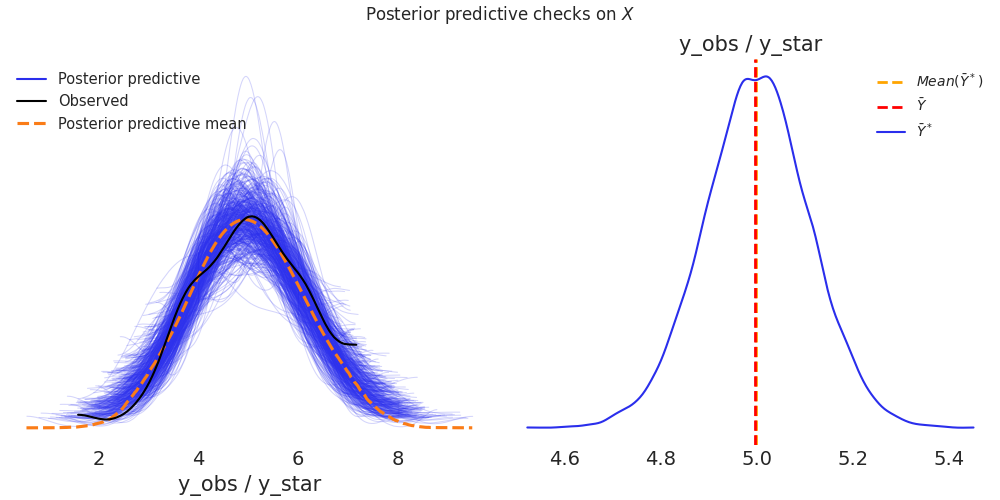
\includegraphics[width=.75\textwidth]{img/ppc_linear}
  \caption{Posterior predictive graphical checks on a fitted model. On the left there is a comparison between the observed distribution of the response variable and the posterior predictive distribution of the approximate sampled responses, while the distribution of the average of the posterior predictive responses is depicted on the right.}\label{fig:ppc}
\end{figure}

\section{Experimental results}\label{sec:results}

We show below the results for 10 random train/test partitions and 5-fold cross-validation to select the parameters \(p\) and \(\eta\).

\subsection{Functional Linear Regression}

\begin{figure}[ht!]
  \centering
  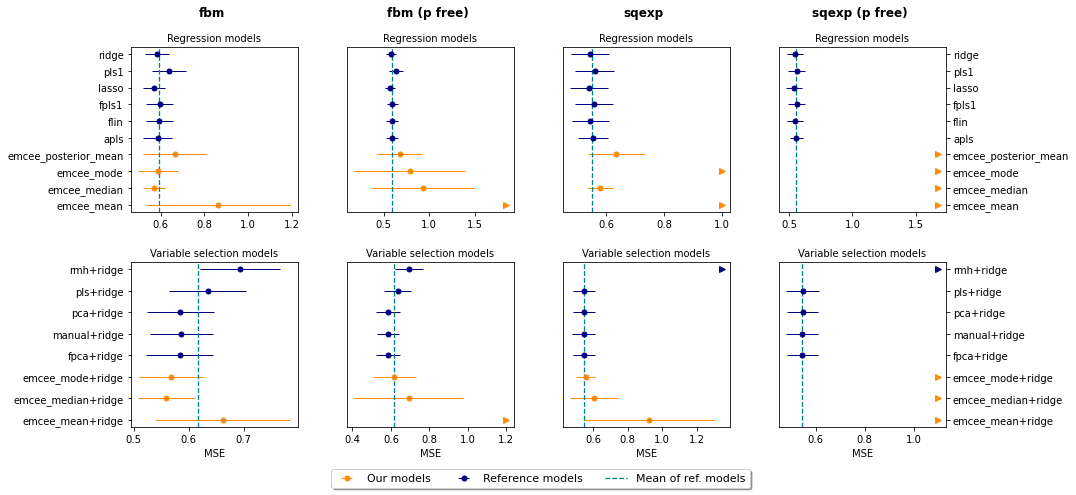
\includegraphics[width=\textwidth]{img/reg_emcee_rkhs}
  \caption{Mean MSE for linear regression with simulated data following an underlying RKHS model.}\label{fig:reg-emcee-rkhs}
\end{figure}

\begin{figure}[ht!]
  \centering
  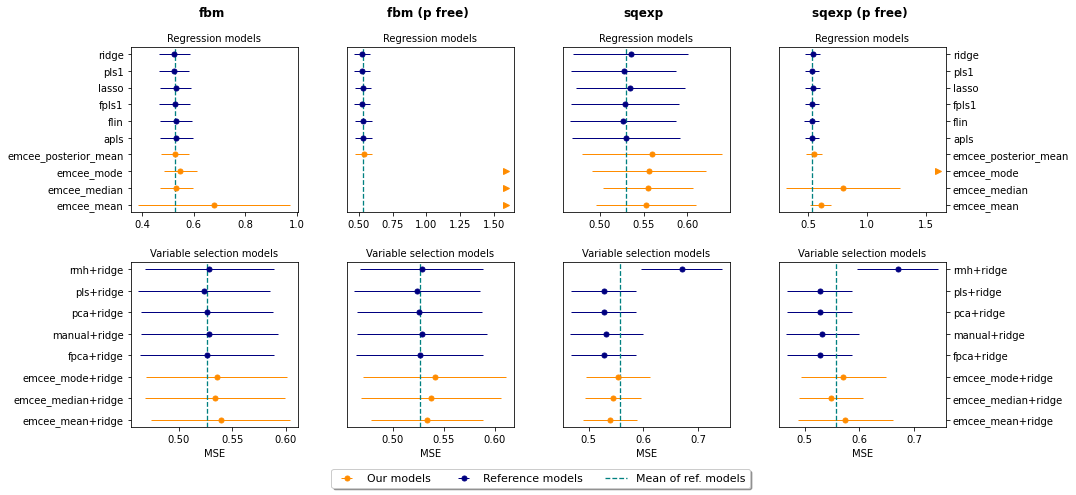
\includegraphics[width=\textwidth]{img/reg_emcee_l2}
  \caption{Mean MSE for linear regression with simulated data following an underlying \(L^2\)-model.}\label{fig:reg-emcee-l2}
\end{figure}

\newpage

\begin{figure}[ht!]
  \centering
  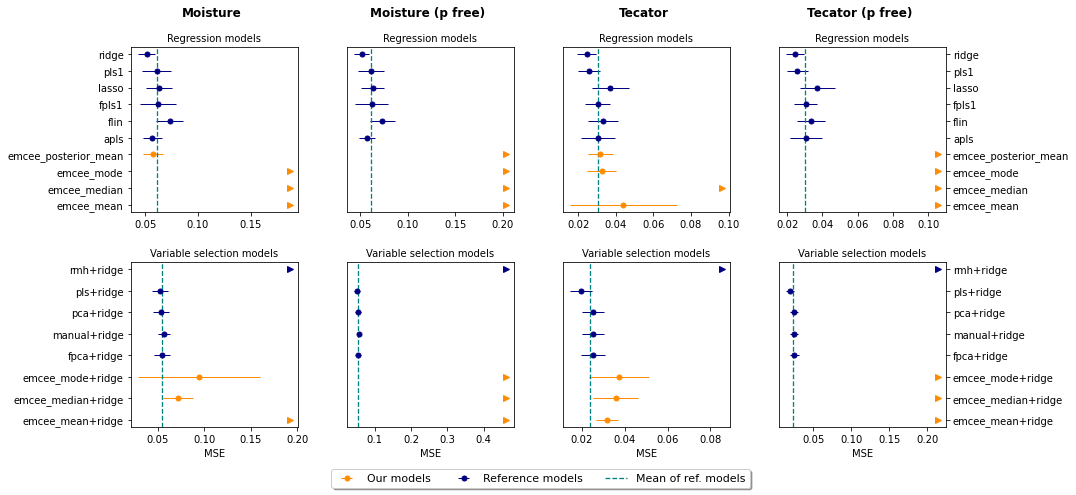
\includegraphics[width=\textwidth]{img/reg_emcee_real}
  \caption{Mean MSE for linear regression with real data sets.}\label{fig:reg-emcee-real}
\end{figure}

\subsection{Functional Logistic Regression}

\begin{figure}[ht!]
  \centering
  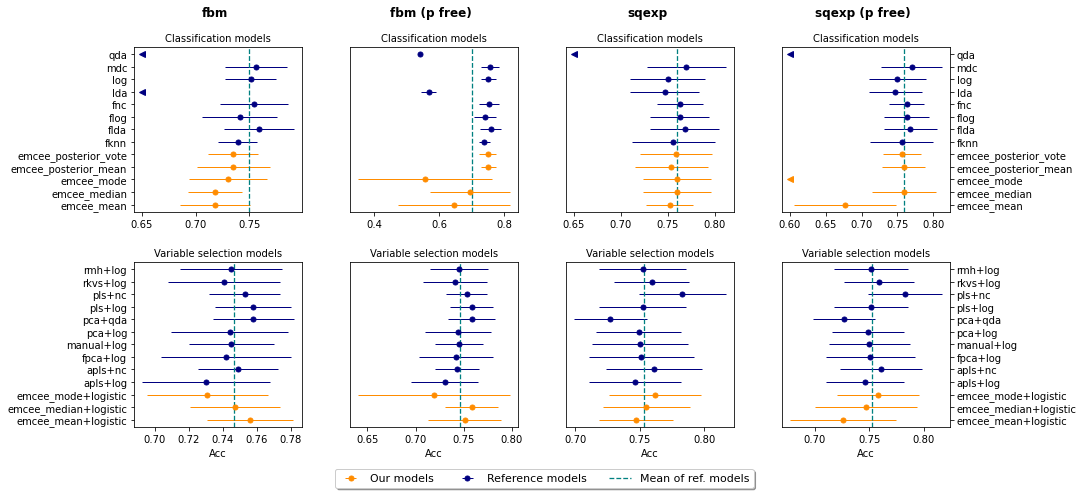
\includegraphics[width=\textwidth]{img/clf_emcee_rkhs}
  \caption{Mean accuracy for logistic regression with simulated data following an underlying RKHS model.}\label{fig:clf-emcee-rkhs}
\end{figure}

\begin{figure}[ht!]
  \centering
  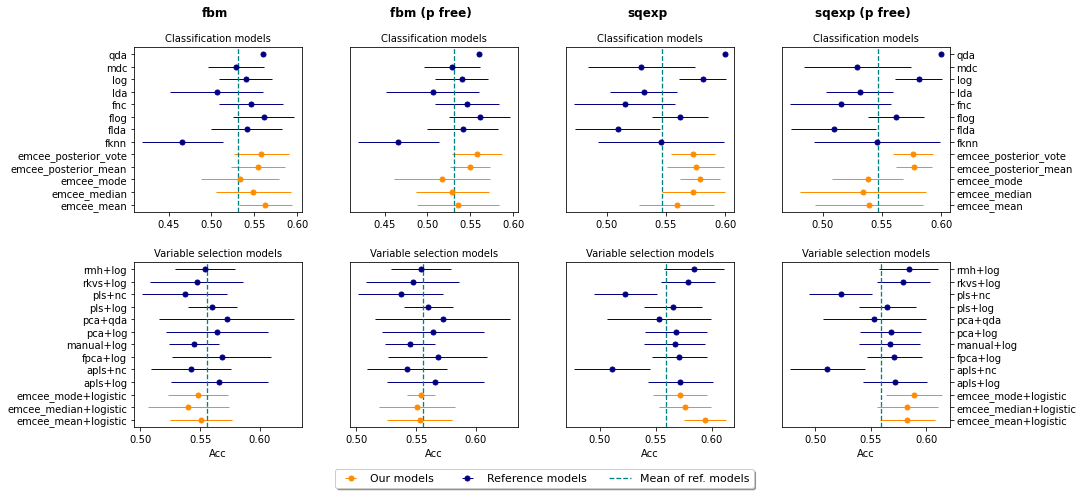
\includegraphics[width=\textwidth]{img/clf_emcee_l2}
  \caption{Mean accuracy for logistic regression with simulated data following an underlying \(L^2\)-model.}\label{fig:clf-emcee-l2}
\end{figure}

\begin{figure}[ht!]
  \centering
  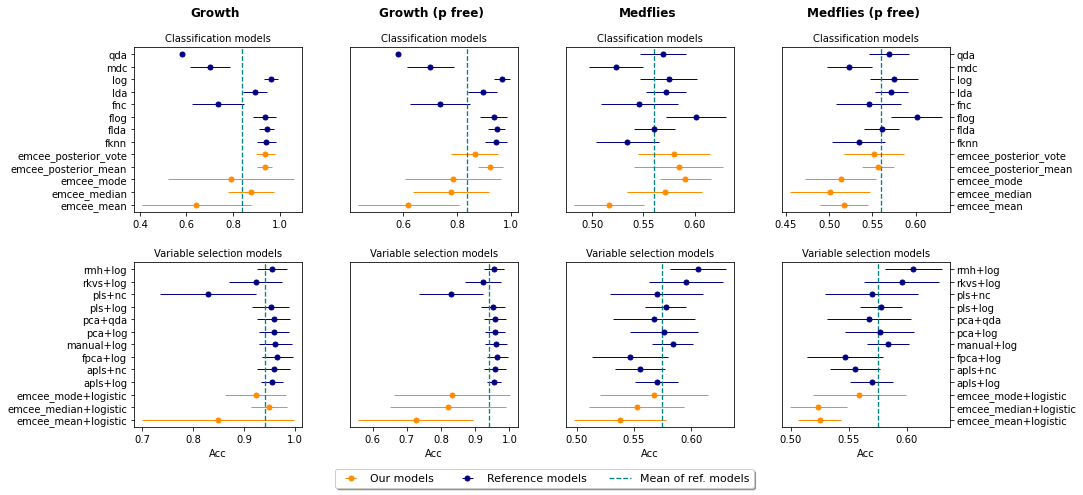
\includegraphics[width=\textwidth]{img/clf_emcee_real}
  \caption{Mean accuracy for logistic regression with real data sets.}\label{fig:clf-emcee-real}
\end{figure}

\newpage

\begin{comment}
  \begin{itemize}
    \item Comentar el método MCMC usado (\textit{emcee}) y por qué (vs. Metropolis u otros basados en gradiente como NUTS). Comentar que se lanzan varias cadenas en paralelo y luego se hace la media, para aumentar estabilidad.
    \item Comentar que se usa el MLE de los parámetros (perturbado) como punto de partida del algoritmo MCMC. Comentar la forma de estimación de MLE (varias iteraciones combinando una búsqueda global con una búsqueda local).
    \item Parámetros comunes de generación de datasets (granularidad de la malla, ...) y de la estrategia de ejecución (dónde se ejecuta, tiempos de ejecución, cuántas veces se repite para eliminar aleatoriedad, ...)
    \item Métricas usadas para medir el error.
    \item Comentar cómo se comparan las distintas estrategias de predicción, cuál parece más estable, etc.
    \item Contar los algoritmos de comparación usados (elegir algunos).
    \item Mostrar tablas de resultados y gráficas. En las gráficas, unificar el eje Y para los mismos modelos, y a ser posible, pintar media y desviación típica de varias ejecuciones (haciendo CV con distintos splits train/test).
    \item Hacer un caso de estudio en el dataset RKHS, midiendo la bondad de las aproximaciones de los instantes de tiempo \(\hat t_j\) a los instantes reales. También estudiar si se recupera el número de componentes subyacente.
    \item En una simulación concreta, mostrar la dependencia del error frente a distintos parámetros del sampler MCMC (por ejemplo, el número de cadenas usadas o el número de iteraciones).
\end{itemize}
\end{comment}

\subsection{Simulation studies}

\subsection{Application to real data}

\section{Conclusion}\label{sec:conclusion}

\begin{supplement}
\stitle{Title of Supplement A}
\sdescription{Short description of Supplement A, with DOI and/or links to additional material (code, ...)}

\begin{comment}
  \begin{itemize}
  \item Comentar el uso de \(\log\sigma\) en lugar de \(\sigma^2\) para que el espacio de búsqueda sea no acotado. Comentar también la posibilidad de transformar \(\tau\) a un espacio no acotado.
  \item Comentar algunas decisiones de implementación: burn-in, thinning a la hora de hacer ppcs, ...
  \item Gráficos de las trazas, de algunas posterioris concretas, etc. También de intervalos de confianza hdi3 y hdi97.
\end{itemize}
\end{comment}

\end{supplement}

\bibliographystyle{bib/ba}
\bibliography{bib/bibliography}

\begin{acks}[Acknowledgments]
The authors wish to acknowledge the computational resources provided by the Centro de Computación Científica-Universidad Autónoma de Madrid (CCC-UAM), which were instrumental in performing the simulations in this paper.
\end{acks}


\end{document}
